%
% LaTeX report template 
%
\documentclass[a4paper,11pt]{article}
\usepackage{graphicx}
\usepackage[english]{babel}
\usepackage{physics}
\usepackage{xcolor}
\usepackage{amsmath}
\usepackage[margin=1.3in]{geometry}
\usepackage{titling}
\usepackage[hang, flushmargin, multiple]{footmisc}
\usepackage[unicode, colorlinks=true, linkcolor=blue, urlcolor=blue, citecolor=blue]{hyperref}
\usepackage{footnotebackref}

\graphicspath{ {images/} }

\setlength\parindent{0pt}

%
\begin{document}
   \droptitle = -30mm
   \title{Notes on: FAQUAD in Quantum Dots}

   \author{David Fernandez Fernandez \\ e-mail: \href{mailto:david.fernandezf03@estudiante.uam.es}{david.fernandezf03@estudiante.uam.es}}
   
   \date{\today}

   \maketitle
   
   \tableofcontents
    

\section{Model}

The system that we study is a quantum dot (QD) array populated with heavy holes in presence of a external magnetic field perpendicular to the dots. Let us first consider the ideal case where there is no SO interaction and therefore the spin is conserved when hopping from one dot to the other. In this case the Hamiltonian is
\begin{equation}
H=\sum_{i\sigma}\varepsilon_{i\sigma}n_{i\sigma}+u\sum_in_{i\uparrow}n_{i\downarrow}-\sum_{i\neq j}\sum_\sigma\tau_{ij}\left(c_{i\sigma}^\dagger c_{j\sigma}+H.c.\right)\; ,
\label{eq:Hubbard_model}
\end{equation}
where $\varepsilon_{i\sigma}$ denoted the energy of the single-particle located in the dot $i$ with spin $\sigma=\uparrow,\downarrow=\pm1/2$. This energy takes into account the bias energy level of the dot and the Zeeman splitting
\begin{equation}
\varepsilon_{i\sigma}=\varepsilon_i+g\mu_B B\sigma\equiv \varepsilon_i+E_Z\sigma\; .
\end{equation}
A typical value of the effective $g$-factor for heavy holes in GaAs could be $g=1.35$. The intradot Coulomb interaction $u$ exist when various particles occupy the same dot. There is also a spin-conserving tunnelling term $\tau$ between adjacent QD's. Finally, the operator $c_{i\sigma}$ ($c_{i\sigma}^{\dagger}$) represents the annihilation (creation) of a hole in the dot $i$ with spin $\sigma$.

\section{\label{sec:DQD}Double Quantum Dot}
The energy spectrum for a double quantum dot array (DQD) populated with two heavy holes is given in Fig~\ref{fig:eigenenergies_2QD_2HH_wo_SOC}, where we have normalized the instant eigenenergies with the Zeeman splitting energy. It's usual to work with an antisymmetric bias gate for each dot where $\varepsilon_R=-\varepsilon_L$, and define the difference as the detuning $\varepsilon\equiv \varepsilon_R-\varepsilon_L$. To obtain this results we have excluded one of the double occupation states $\ket{S(2,0)}$, which is motivated by the setups where it's energy is much higher.
\begin{figure}[!htbp]
	\centering
	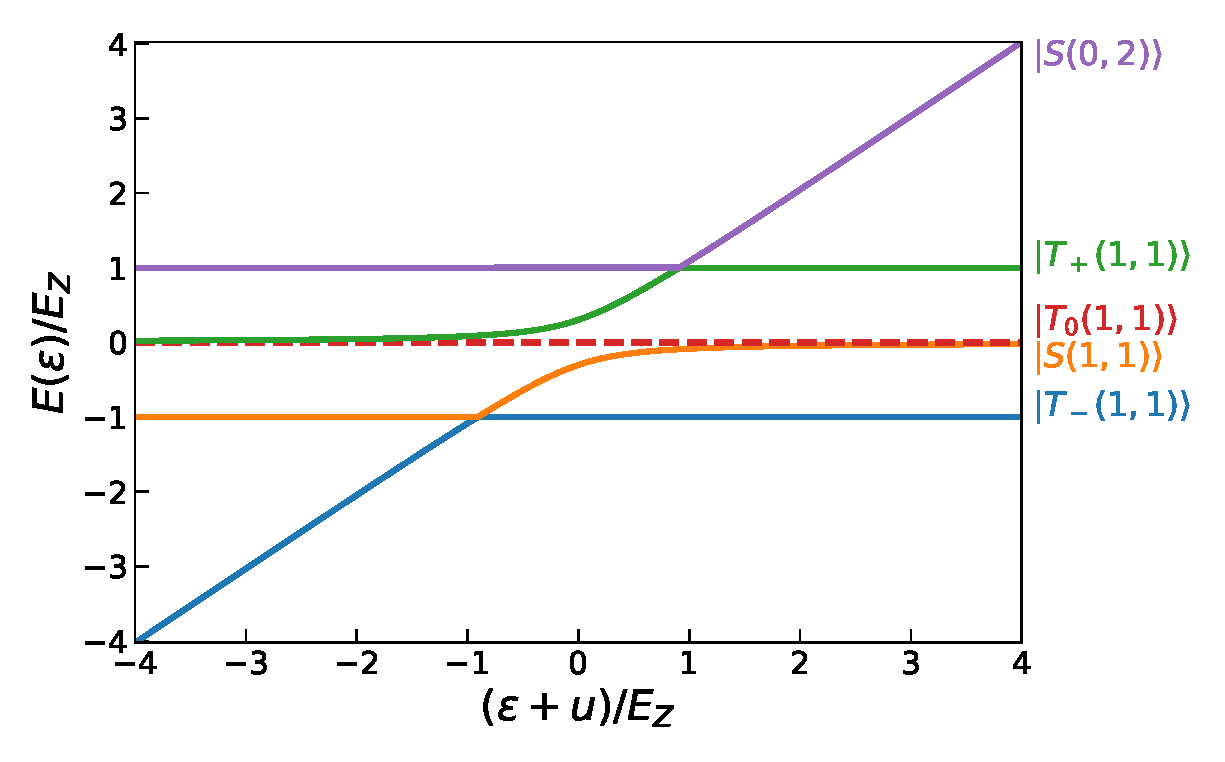
\includegraphics[width=0.8\linewidth]{eigenenergies_2QD_2HH_wo_SOC.eps}
	\caption{Energy spectrum for the system of a double quantum dot array populated with two heavy holes without spin orbit coupling. The parameters used are $B=0.015$~T, $E_Z=1.17\; \mu$eV, $\tau=0.25\; \mu$eV and $u=2$ meV.}
	\label{fig:eigenenergies_2QD_2HH_wo_SOC}
\end{figure}

We are only interested in the subspace formed by the two singlets states $\ket{S(1,1)}$, $\ket{S(0,2)}$, and the least energetic triplet estate $\ket{T_-(1,1)}$. With this the Hamiltonian can be easily written with the matrix
\begin{equation}
	H=\bordermatrix{~ & \ket{T_-(1,1)} & \ket{S(1,1)} & \ket{S(0,2)}\cr
		~ & -E_Z & 0 & 0 \cr
		~ & 0 & 0 & \sqrt{2}\tau \cr
		~ & 0 & \sqrt{2}\tau & \varepsilon+u \cr}\; .
\end{equation}
In order to couple the singlets and the triplet we can introduce two new terms, the Dresselhaus SOC and the Rashba SOC
\begin{equation}
	\begin{split}
	H_D&=\beta(\sigma_+p_-m_+p_--\sigma_-p_+p_-p_+)\\
	H_R&=i\alpha E_\perp (\sigma_+p_-^3-\sigma_+p_-^3)\; .
	\end{split}
\end{equation}
The ladder operators are defined by
\begin{equation}
	\begin{split}
	p_+\equiv p_x+ip_y\;, \quad p_-\equiv p_x-ip_y\;, 
	\end{split}
\end{equation}
where the momentum $p_x=-i\hbar \partial/\partial x$ and similar for $p_y$. To keep the computations as simpler as possible we take both SOC parameters to be equal $\beta=\alpha E_\perp$. The two new coupling terms are defined as
\begin{equation}
	\begin{split}
	\lambda_1&=\bra{T_-(1,1)}H_D+H_S\ket{S(1,1)}\\
	\lambda_2&=\bra{T_-(1,1)}H_D+H_S\ket{S(0,2)}\; .
	\end{split}
\end{equation}
To obtain an analytical expression for this two terms we can impose the single hole orbital functions with Gaussian shapes centered at each dot
\begin{equation}
	\psi_i=\frac{1}{l}\sqrt{\frac{2}{\pi}}\exp(-\frac{(x-x_i)^2+y^2}{l^2})\; ,
\end{equation} 
where the dot lies in the $x$ axis, $d$ is the interdot distance $x_1=-x_2=d/2$, and $l$ is the extent of the wave function. After integration we obtain the expressions
\begin{equation}
	\begin{split}
	\lambda_1&=\frac{8\alpha E_\perp d}{l^4}\exp(-d^2/l^2)\\
	\lambda_2&=\frac{4\sqrt{2}\alpha E_\perp d}{l^4}\exp(-d^2/2l^2)\; .
	\end{split}
\end{equation}
Choosing $l=d/3$ we observe that $\lambda_1/\lambda_2\approx 1/100$, being the coupling with the double occupation singlet states stronger. An analytical solution for the instant eigenstates is too complex, but we can solve it numerically, obtaining the energy spectrum shown in Fig~\ref{fig:eigenenergies_2QD_2HH_w_SOC}.
\begin{figure}[!htbp]
	\centering
	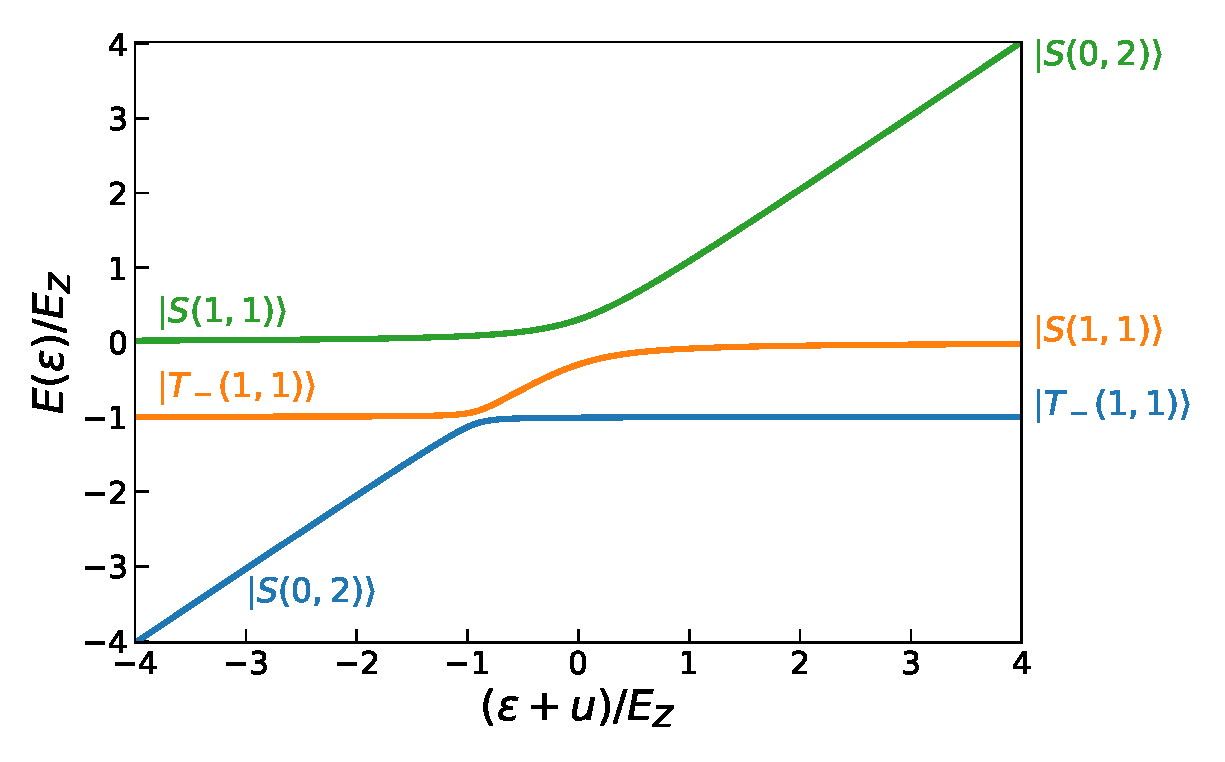
\includegraphics[width=0.8\linewidth]{eigenenergies_2QD_2HH_w_SOC.eps}
	\caption{Three lowest energies for the system of a double quantum dot array populated with two heavy holes in presence spin orbit coupling. The parameters used are $B=0.015$~T, $E_Z=1.17\; \mu$eV, $\tau=0.25\; \mu$eV, $\lambda_1=0.001\; \mu$eV, $\lambda_2=0.1\; \mu$eV and $u=2$ meV.}
	\label{fig:eigenenergies_2QD_2HH_w_SOC}
\end{figure}
Our task is to pass from $\ket{T_-(1,1)}$ to $S(1,1)$ with the minimum possible occupation of $S(0,2)$. The reason is that we want to reduce as much as possible charge noise. We have not include any term in the Hamiltonian that flip the spin of the hole without ``jumping" to some other qubit, so the only possible transition allowed is
\begin{equation}
	\ket{\downarrow,\downarrow}\rightarrow \ket{0,\uparrow\downarrow} \rightarrow \frac{1}{\sqrt{2}}\left(\ket{\uparrow,\downarrow}-\ket{\downarrow,\uparrow}\right)\; .
\end{equation}
There exist some quasi adiabatic techniques that take advantage of the existence of a dark-state which has no weight in the intermediate step. To check if this is also the case for our system we can compute numerically the instant eigenvectors and extracting the probability to occupy the double occupation singlet state Fig~\ref{fig:occupation_middle_state}. Here we have plotted the value $|\braket{\psi_2}{S(0,2)}|^2$ where $\ket{\psi_2}$ correspond to the state in which we are interested (orange line in Fig~(\ref{fig:eigenenergies_2QD_2HH_w_SOC})).
\begin{figure}[!htbp]
	\centering
	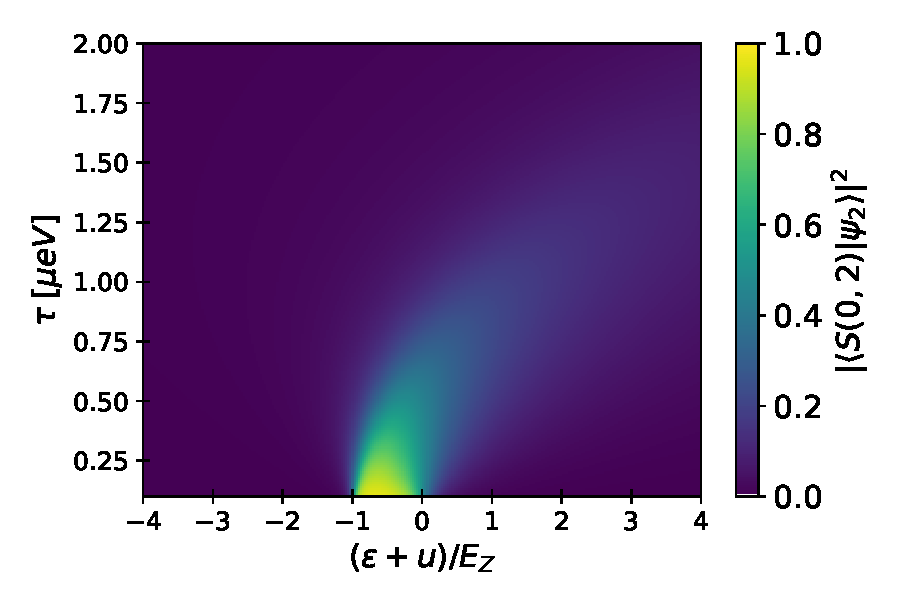
\includegraphics[width=0.6\linewidth]{occupation_middle_state.eps}
	\caption{Contribution of the double occupation singlet state in the instant eigenstate $\ket{\psi_2}$ in terms of the detuning and the spin conserving tunnelling parameter $\tau$. For the SOC parameters we have set $\lambda_1=\lambda_2/100$ and $\lambda_2=0.25\tau$.}
	\label{fig:occupation_middle_state}
\end{figure}

To study the dependency with the tunnelling we have assumed that both the spin-flip and spin-conserving rates are proportional to each other $\lambda_i\propto \tau$, specifically we have used $\lambda_2=0.25\tau$ and $\lambda_1=\lambda_2/100$. If we want to make a transition between the lowest energy triplet and the single occupation singlet we must go from $(\varepsilon(t_0)+u)/E_Z=-4$ to $(\varepsilon(t_f)+u)/E_Z=4$, this means that there is no dark state that does not populate the $\ket{S(0,2)}$ in the range of detuning in which we are interest unless the tunnelling parameters are high enough. This is why we will try to apply the FAst QUasi ADiabatic (FAQUAD) protocol in the next section.

\section{FAQUAD}
The standard adiabaticity parameter is imposed to be constant, as
\begin{equation}
	\hbar\abs{\frac{\braket{\phi_1(t)}{\partial_t\phi_2(t)}}{E_1(t)-E_2(t)}}=c\; .
\end{equation}
This is only the case in which there are two states. If we a multilevel system the above equation is rewritten as
\begin{equation}
	\hbar \sum _{k\neq i}\abs{\frac{\braket{\phi_i(t)}{\partial_t\phi_k(t)}}{E_i(t)-E_k(t)}}=c\; ,
\end{equation}
where the index $i$ denote the state in which we initialize the system, in our case it will be $\ket{\phi_i(t)}=\ket{T_-(1,1)}$. Using the chain rule we can write $\partial_t=\partial_\varepsilon \dot{\varepsilon}$ and the adiabatic condition is then
\begin{equation}
	\dot{\varepsilon}=\frac{c}{\hbar}\left(\sum _{k\neq i}\abs{\frac{\braket{\phi_i(t)}{\partial_\varepsilon\phi_k(t)}}{E_i(t)-E_k(t)}}\right)^{-1}\; .
	\label{eq:detuning_EDO}
\end{equation}
We can rescale the total operation time $t_f$ to $s\equiv t/t_f$ and define $\tilde{c}\equiv ct_f$, allowing us to write
\begin{equation}
	\tilde{c}=\int_{\varepsilon(0)}^{\varepsilon(t_f)}d\varepsilon\left(\sum _{k\neq i}\abs{\frac{\braket{\phi_i(t)}{\partial_\varepsilon\phi_k(t)}}{E_i(t)-E_k(t)}}\right)\; , 
\end{equation}
what can be easily computed numerically, obtaining a value of $\tilde{c}=3.79$ ns, so with typical times of $t_f\sim 10$ ns the adiabaticity parameter obtained is $c\sim 0.4< 1$ fulfilling the adiabatic condition. Once we have obtained the value for this parameters, which will remain constant, we can numerically solve the EDO for the evolution of the detuning Eq.~(\ref{eq:detuning_EDO}). The result is shown in Fig.~\ref{fig:FAQUAD_detuning_2QD_2HH}, the dependency of this parameter with $s=t/t_f$ is plotted in a), while the derivative is represented in b) in terms of the detuning. We observe that when we reach the two avoided crossings the rate of change in the detuning decreases significantly, allowing an adiabatic passage, while in the rest of the point the velocity increases in order to speed up the transfer process.
\begin{figure}[!htbp]
	\centering
	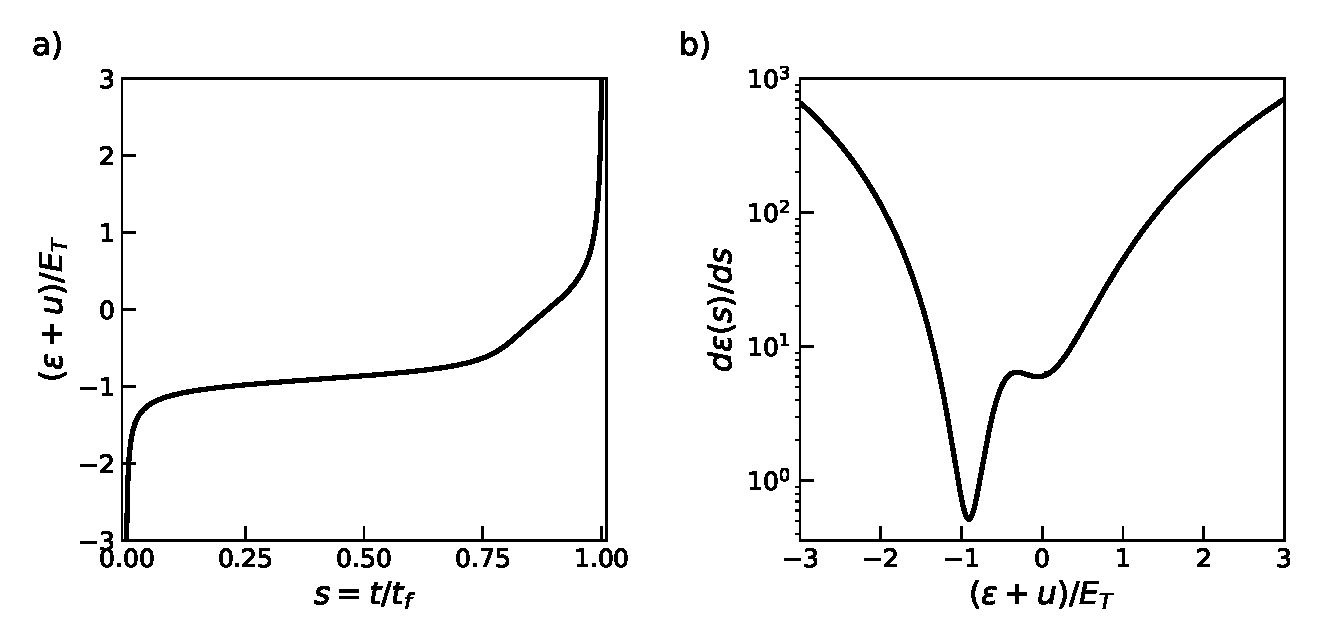
\includegraphics[width=1\linewidth]{FAQUAD_detuning_2QD_2HH.eps}
	\caption{Result obtained for the detuning after applying the FAQUAD protocol to the system of DQD populated with two HH. In a) the dependence of the detuning in terms of the adimensional parameters $s$. In b) the slope of the detuning $\varepsilon^\prime\equiv d \varepsilon/d s$ in terms of the detuning.}
	\label{fig:FAQUAD_detuning_2QD_2HH}
\end{figure}

We define the fidelity of this protocol as
\begin{equation}
	\mathcal{F}\equiv \abs{\braket{S(1,1)}{\psi(t_f)}}^2\; .
\end{equation}
Computing this fidelity for different total times $t_f$ we obtain the results shown in Fig.~\ref{fig:FAQUAD_2QD_Results}.
\begin{figure}[!htbp]
	\centering
	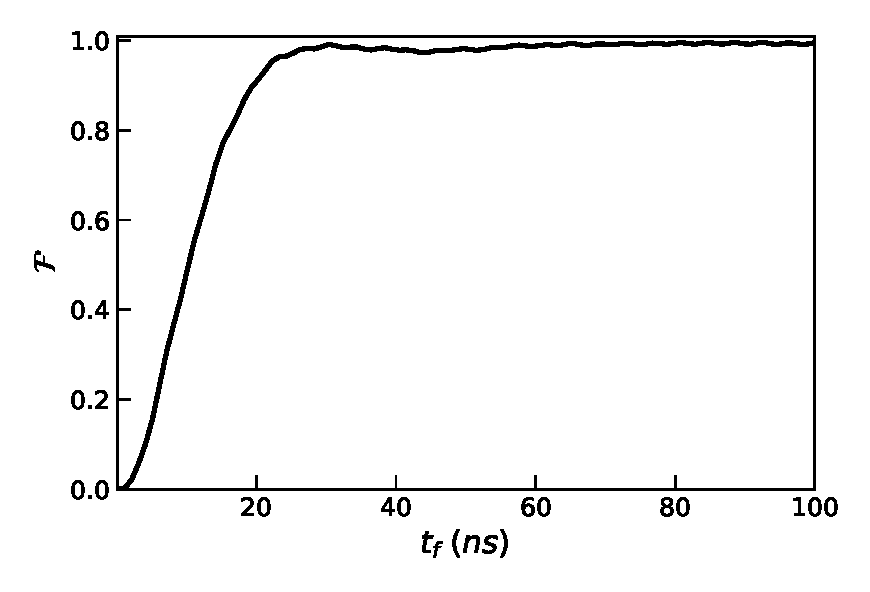
\includegraphics[width=0.7\linewidth]{FAQUAD_2QD_Results.eps}
	\caption{Result for the fidelity in terms of the total time of the protocol.}
	\label{fig:FAQUAD_2QD_Results}
\end{figure}

We can observe that the fidelity shows it's typical FAQUAD protocol behaviour, reaching a value close to the unit for large enough final times. The first peak is reached at $t_f=30.4$ ns, with a fidelity of $\mathcal{F}=0.992$. In Fig.~\ref{fig:states_evolution} we plot the time evolution for the three different states for this value for the total operation time. We observe that the desired final state is obtained, but in the intermediate times the population for the $S(0,2)$ state is too high.
\begin{figure}[!htbp]
	\centering
	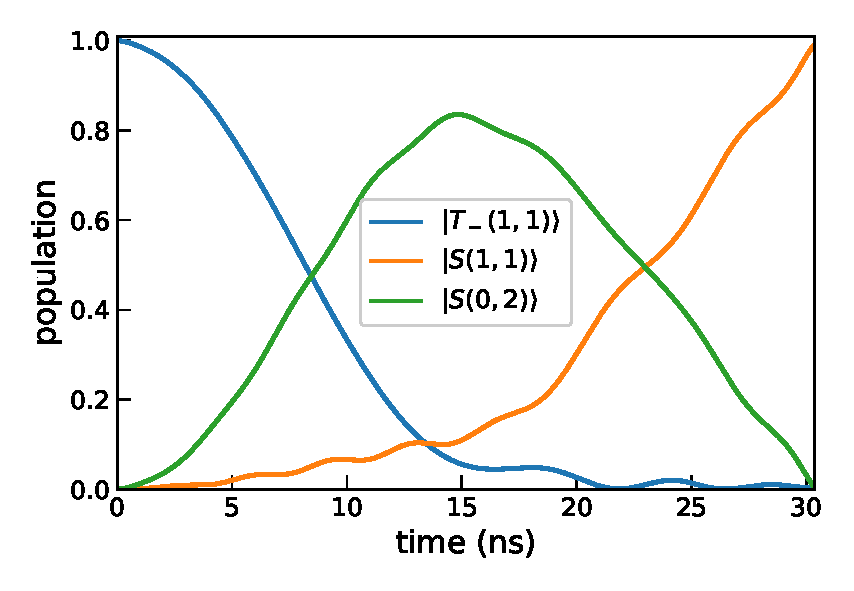
\includegraphics[width=0.7\linewidth]{states_evolution.eps}
	\caption{Evolution of the different states for the final time of $t_f=30.4$ ns and a fidelity $\mathcal{F}=0.992$.}
	\label{fig:states_evolution}
\end{figure}


\appendix
\section{Equivalence between SOC Models}
In Sec.~\ref{sec:DQD} we have introduced the SOC with the terms
\begin{equation}
	\begin{split}
	\lambda_1&=\bra{T_-(1,1)}H_D+H_S\ket{S(1,1)}\\
	\lambda_2&=\bra{T_-(1,1)}H_D+H_S\ket{S(0,2)}\; ,
	\end{split}
\end{equation}
and the total Hamiltonian is then written as
\begin{equation}
H=\bordermatrix{~ & \ket{T_-(1,1)} & \ket{S(1,1)} & \ket{S(0,2)}\cr
	~ & -E_Z & \lambda_1 & \lambda_2 \cr
	~ & \lambda_1 & 0 & \sqrt{2}\tau \cr
	~ & \lambda_2 & \sqrt{2}\tau & \varepsilon+u \cr}\; .
\label{eq:Hamiltonian_Yue}
\end{equation}
Supposing Gaussian shapes for the wave functions, and with some given parameters we have obtained that $\lambda_1\ll\lambda_2$. In other references \cite{Bogan2018} the result is a little different. Using the Loewdin procedure we can redefine our basis orbitals as $\ket{\overline{L}}=\ket{L}-\frac{1}{2}S\ket{R}$ and $\ket{\overline{R}}=\ket{R}-\frac{1}{2}S\ket{L}$, where $S=\exp(-d^2/2l^2)$ is the overlapping of the original orbitals. Using this we obtain the expression for the spin flip tunnelling
\begin{equation}
	\bra{\overline{L}\uparrow}H_D+H_S\ket{\overline{R}\downarrow}=-\alpha E_\perp \frac{d^3}{l^6}\exp(-\frac{d^2}{2l^2})-i\beta\left(\frac{4d}{l^4}-\frac{d^3}{l^6}\right)\exp(-\frac{d^2}{2l^2})\; .
\end{equation}
We will define this matrix element as $\bra{\overline{L}\uparrow}H_{\text{SOC}}\ket{\overline{R}\downarrow}\equiv -it_Fe^{i\delta}$, where the phase depends on the relative strength of the Rashba and Dresselhaus SOC. With this the Hamiltonian, in the atomic base, is written as
\begin{equation}
H_{\text{atomic}}=\bordermatrix{~ & \ket{\uparrow,\uparrow} & \ket{\uparrow,\downarrow} & \ket{\downarrow,\uparrow} & \ket{\downarrow,\downarrow} & \ket{0,\uparrow\downarrow}\cr
	~ & E_Z   			 & 0     & 0    & 0    			   & it_Fe^{-i\delta}  \cr
	~ & 0     			 & 0     & 0    & 0    			   & -\tau  		  	\cr
	~ & 0     			 & 0     & 0    & 0    			   & \tau 		  		\cr
	~ & 0     			 & 0     & 0    & -E_Z 			   & -it_Fe^{i\delta}   \cr
	~ & -it_Fe^{i\delta} & -\tau & \tau & it_Fe^{-i\delta} & \varepsilon+u}\; .
\end{equation}
Just by changing to the molecular base we obtain the matrix
\begin{equation}
H_{\text{molecular}}=\bordermatrix{~ & \ket{T_+(1,1)} & \ket{T_0(1,1)} & \ket{T_-(1,1)} & \ket{S(1,1)} & \ket{S(0,2)}\cr
	~ & E_Z   			 & 0     & 0      			  & 0    		   & it_Fe^{-i\delta}	 \cr
	~ & 0     			 & 0     & 0      			  & 0    		   & 0 		  	 		 \cr
	~ & 0     			 & 0     & -E_Z   			  & 0    		   & -it_Fe^{i\delta}    \cr
	~ & 0     			 & 0     & 0      			  & 0    		   & -\sqrt{2}\tau 		 \cr
	~ & -it_Fe^{i\delta} & 0     & it_Fe^{-i\delta}   & -\sqrt{2}\tau  & \varepsilon+u}\; .
\end{equation} We can restrict ourselves to the subspace $\ket{T_-(1,1)}, \ket{S(1,1)}, \ket{S(0,2)}$, computing the characteristic polynomial we have the equation
\begin{equation}
	(\varepsilon+u-x)x^2+x((\varepsilon+u-x)E_Z+t_F^2)+2(x+E_Z)\tau^2\; ,
\end{equation}
which does not depend on the exact phase of the spin flip tunnelling, so we can set it to zero $\delta=0$. With this we can write the Hamiltonian for the sub-space in which we are interested as
\begin{equation}
H=\bordermatrix{~ & \ket{T_-(1,1)} & \ket{S(1,1)} & \ket{S(0,2)}\cr
	~ & -E_Z & 0 & -it_F \cr
	~ & 0 & 0 & \sqrt{2}\tau \cr
	~ & it_F & \sqrt{2}\tau & \varepsilon+u \cr}\; .
\end{equation}
This is indeed the same Hamiltonian that the one shown in Eq.~(\ref{eq:Hamiltonian_Yue}) under $\lambda_1\rightarrow 0$ and $\lambda_2\rightarrow -it_F$.


\bibliographystyle{IEEEtran}
\bibliography{references}

\end{document}

